\begin{figure*}[t!]
	\centering
	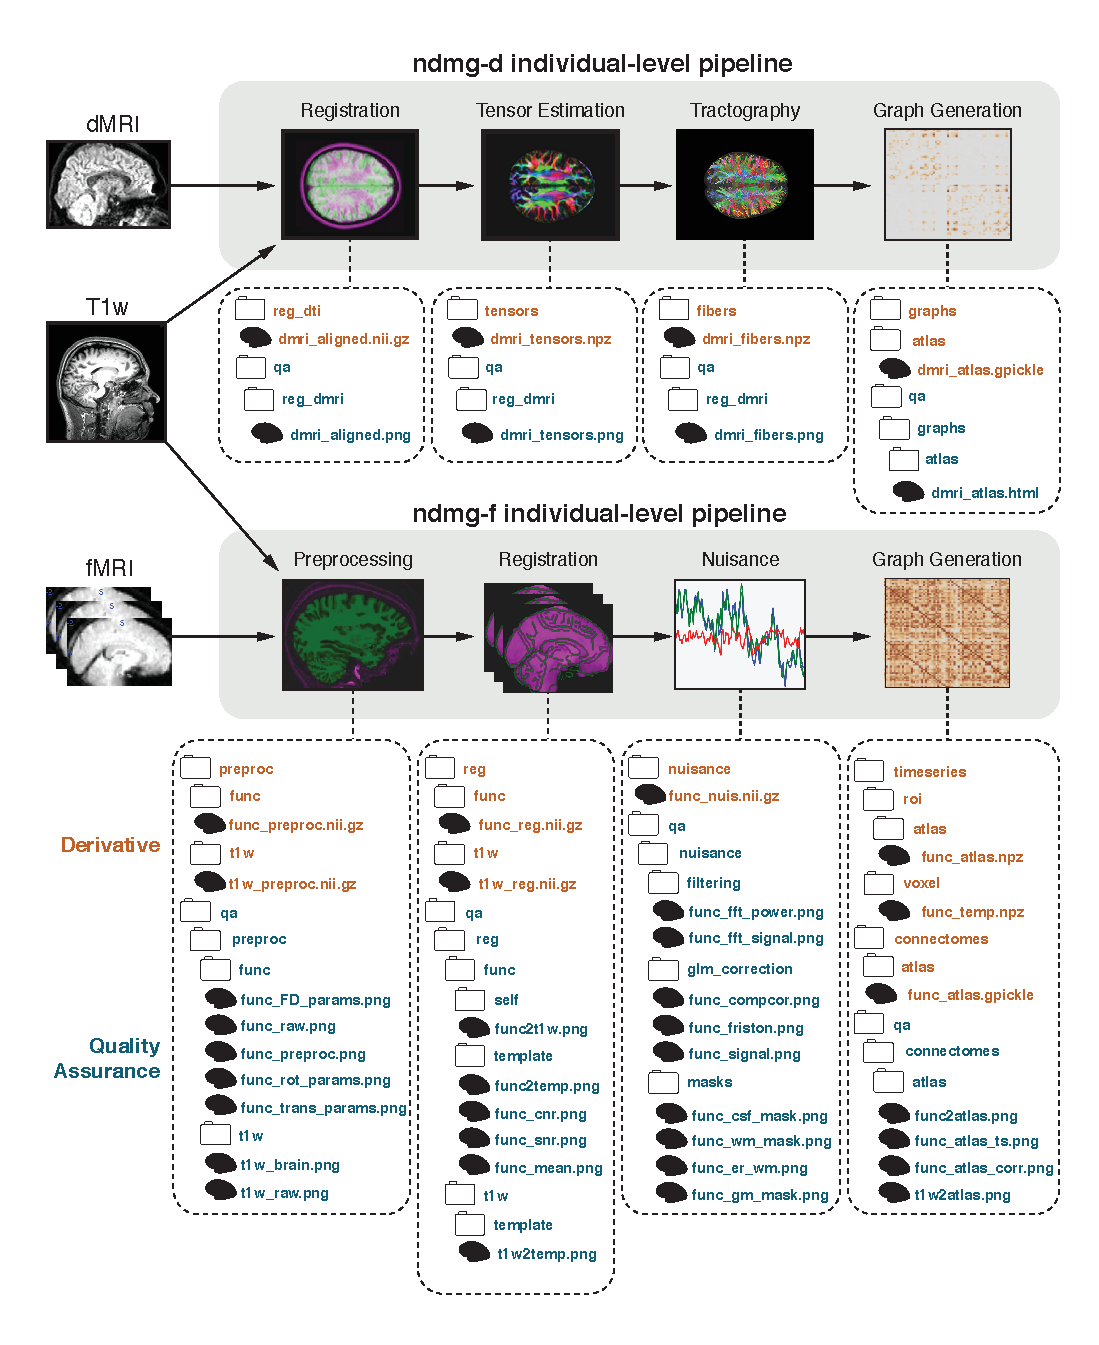
\includegraphics[width=0.9\textwidth]{./figs/ndmg_pipeline.pdf}
    \caption{\textbf{Individual Level Pipeline}
  The individual-level  \ndmg~pipeline has two sub-pipelines:  (1) \ndmgd~transforms raw dMRI data into sparse structural connectomes, and (2) \ndmgf~transforms raw fMRI data into dense functional connectomes.  Each sub-pipeline consists of four key steps, and each step generates both data derivatives and quality assurance figures to enable both qualitative assessments and quantitative comparisons (see~\ref{app:dpipe} and~\ref{app:fpipe} for details).  
%  as seen in the top. \ndmgd~consists of four main steps: registration, tensor estimation, tractography, and graph generation. Simiarly, the subject-level of the \ndmgf~pipeline transforms raw functional MRI data into structural connectomes, as seen in the bottom. \ndmgf~consists of four main steps: preprocessing, registration, nuisance-correction, and graph generation.
%  At each stage, \ndmg~produces both data derivatives and quality assurance figures of the derivative, as illustrated.
}
	\label{fig:ndmgpipeline}
\end{figure*}